\documentclass[10pt]{scrreprt}
\usepackage[a4paper, top=30mm, left=25mm, right=25mm, bottom=30mm]{geometry}
\usepackage[utf8]{inputenc}

\usepackage[Bjornstrup]{fncychap}
\usepackage{pdfpages}
\usepackage{ngerman}
\usepackage{graphicx}
\usepackage{epstopdf}
\usepackage{etoolbox}
\usepackage{wrapfig}
\usepackage{enumitem}
\usepackage{tabu}
\usepackage{amsmath}
\usepackage{url}
\usepackage{numprint}
\usepackage{longtable}
\usepackage{caption}
 \usepackage{rotating}
\usepackage{array}
\usepackage{listings}
\usepackage{amssymb}
\usepackage{multirow}
\usepackage{textcomp}
\usepackage{calc}
\usepackage{ulem}
\usepackage[table]{xcolor}
%\usepackage{hyperref}
%\hypersetup{%
%  colorlinks=false,%
%  linkcolor=blue,%
%  citecolor=blue,%
%  unicode%
%}
\usepackage{mathptmx}
\usepackage{courier}
\usepackage{amssymb}

\renewcommand{\em}{\sffamily\bfseries}
\renewcommand{\bf}{\sffamily\bfseries}
\newcommand{\hyperlink}[2]{#1}

\makeatletter
\patchcmd{\@makechapterhead}{\vspace*{50\p@}}{\vspace*{-20\p@}}{}{}
\patchcmd{\@makeschapterhead}{\vspace*{50\p@}}{\vspace*{7\p@}}{}{}
\patchcmd{\DOTIS}{\vskip 40\p@}{\vskip -12\p@} 
\makeatother
  
\captionsetup[figure]{labelfont={sf,bf},textfont={sf}}
\deffootnotemark{[\thefootnotemark]}
\deffootnote{1.5em}{1em}{[\thefootnotemark] }
\setlength{\parindent}{0pt}
\renewcommand{\labelitemi}{ \raisebox{0.3ex}{\small$\blacktriangleright$} }
\renewcommand{\labelitemii}{ \raisebox{0.3ex}{\small$\triangleright$} }
\lstset{language=Java}

\newcommand{\sfbf}[1]{\textbf{\sffamily #1}}
\newcommand{\sfit}[1]{\textit{\sffamily #1}}
\newcommand{\W}{\sfbf{W}}
\newcommand{\ziel}[1]{{\fontsize{9.5}{11}\textsf{/#1/}}}
\newcommand{\ziellabel}{Z}
\newcommand{\muss}{\renewcommand{\labelenumi}{\textbf{\ziel{\ziellabel\numprint{\theenumi}0}}}}
\newcommand{\wunsch}{\renewcommand{\labelenumi}{\textbf{\ziel{\ziellabel\numprint{\theenumi}0W}}}}
\newcommand{\JoglEarth}{\raisebox{-1.2mm}{
\includegraphics[scale=0.33]{Logo-Text.eps}} }
\newcommand{\textref}[1]{\mbox{\raisebox{0.1ex}{\small$\rightarrow$ }\textit{#1}}}

\newenvironment{details}[1][6pt]{%
  \parskip#1 \parindent6mm \raggedright%
  \def\item{\par\ignorespaces\hangindent=5mm \hangafter1}}{%
  \par\ignorespaces} 
  
 
\begin{document}

\thispagestyle{empty}
\sffamily
 
\title{Spezifikation}

\begin{figure}
\begin{flushright}
	
\includegraphics[scale=0.4]{uniLogo.eps}
\vspace{2.0 cm}
\end{flushright}
\end{figure}

\begin{center}
\vspace{2.0 cm}
{\LARGE SEP – Wintersemester 2013/14}

\vspace{1.0 cm}
\textbf{{\Huge Implementierungsbericht}}

\vspace{0.4 cm}
\begin{figure}[!htb]
\begin{center}
	%
\includegraphics[scale=1.0]{projektLogo.eps}
	
\includegraphics[scale=1.5]{Logo-Print.eps}
\end{center}
\end{figure}

\vspace{0.2 cm}
\textbf{{\huge OpenStreetMap: Die Welt in 3D}}

\vspace{1.5 cm}
29.11.2013

\vspace{0.5 cm}
Version: 1.1

\vspace{1.5 cm}
{\Large Projektbetreuer: Peter Barth}

\vspace{1.5 cm}
\begin{tabular}{|c|c|c|}
\hline 
\rule[-1ex]{0pt}{4ex} \textbf{Phase} & \textbf{Verantwortlicher} & \textbf{E-Mail Adresse} \\ 
\hline  \hline
\rule[-1ex]{0pt}{4ex} Pflichtenheft & Gabriele Haas & haasgab@fim.uni-passau.de \\ 
\hline  \hline
\rule[-1ex]{0pt}{4ex} Entwurf & Thomas Eder & ederthom@fim.uni-passau.de \\ 
\hline  \hline
\rule[-1ex]{0pt}{4ex} Spezifikation & Christof Blauberger & blauberg@fim.uni-passau.de \\ 
\hline  \hline
\rule[-1ex]{0pt}{4ex} Implementierung & Fabian Knorr & knorrfab@fim.uni-passau.de \\ 
\hline \hline 
\rule[-1ex]{0pt}{4ex} Testing & Constantin Wenger & wengerco@fim.uni-passau.de \\ 
\hline  \hline
\rule[-1ex]{0pt}{4ex} Präsentation & Sebastian Reichl & reichlse@fim.uni-passau.de \\ 
\hline 
\end{tabular}

\end{center}


\pagebreak
\rmfamily
\tableofcontents

\chapter{Einleitung}

In der Implementierungsphase wurde die Spezifikation von \JoglEarth gemäß dem Implementierungsplan umgesetzt. \\[5mm]
Während der Implementierung wurden naturgemäß Schwächen des Designs und der Spezifikation festgestellt, weswegen außerplanmäßig ein größerer \textit{Refactoring}-Arbeitsschritt am Ende der Entwicklung notwendig wurde. \\[5mm]
In diesem Dokument wird daher zunächst der Implementierungsplan wiedergegeben, anschließend einige Entwicklerstatistiken aufgezählt und anschließend wesentliche Änderungen gegenüber dem Entwurfs- und Spezifikationsdokument dargestellt.


\chapter{Implementierungsplan}

Da die Umsetzung der Enumerations und Interfaces bereits während der Spezifikationsphase erfolgt ist, waren nur noch die Implementierung der Klassen auf Arbeitspaktete zu verteilen.

Der Implementierungsplan besteht aus drei Meilensteinen. Im folgenden wird eine Übersicht über den Inhalt der einzelnen Pakete gegeben, anschließend folgt der Plan als Gantt-Diagramm.\\[3mm]
Die \JoglEarth -Entwickler wurden in Programmierteams eingeteilt; Die Zugehörigkeit wird durch die Färbung der Balken im Diagramm wiedergegeben.

\vspace{3mm}
\begin{center}
\begin{tabular}{|c|c|}
\hline
\rule[-1ex]{0pt}{4ex} \textbf{Balkenfarbe} & \textbf{Team} \\
\hline
\hline
\rule[-1ex]{0pt}{4ex} Blau & Constantin Wenger\\
\hline
\rule[-1ex]{0pt}{4ex} Lila & Christof Blauberger \& Gabriele Haas\\
\hline
\rule[-1ex]{0pt}{4ex} Grün & Fabian Knorr, Thomas Eder \& Sebastian Reichl\\
\hline
\end{tabular}
\end{center}

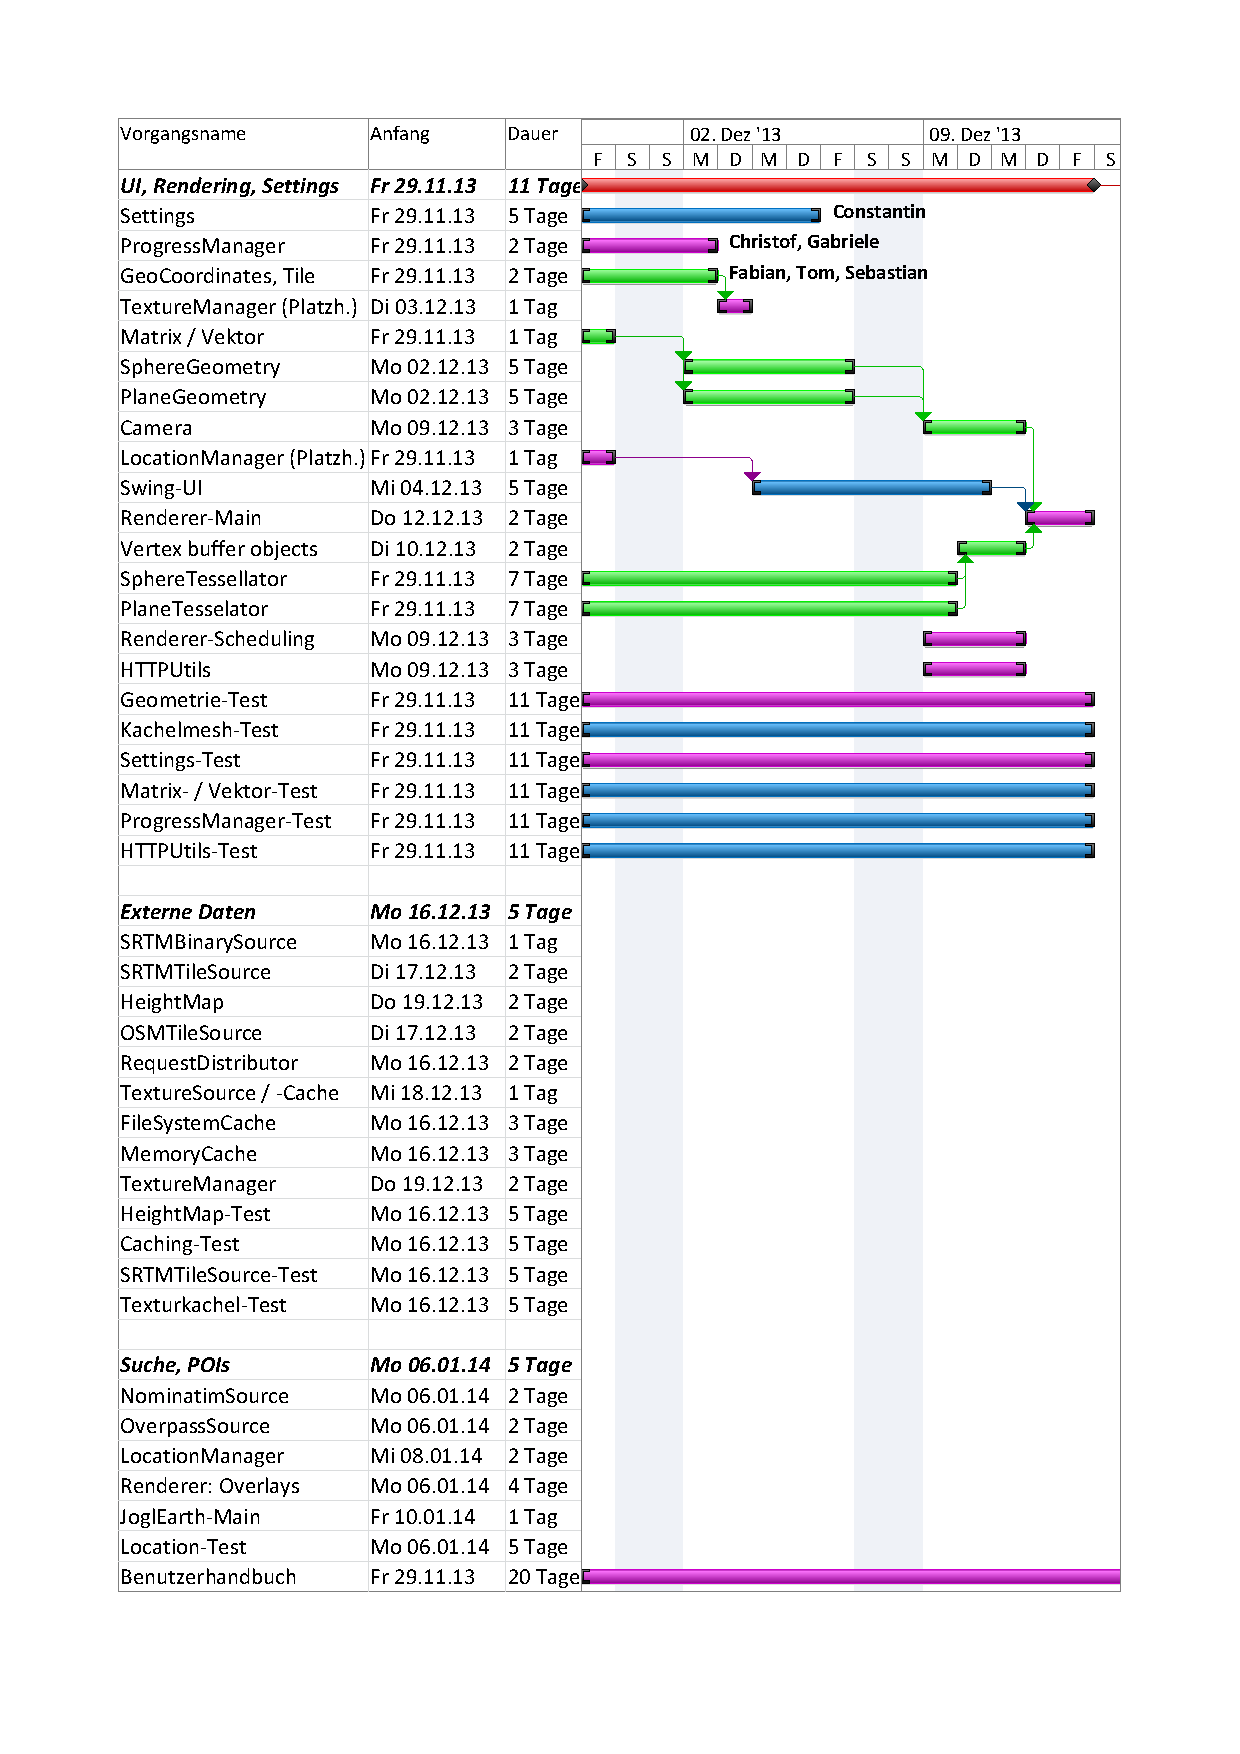
\includepdf[pages={1-3}]{Gantt_JoglEarth.pdf}


\chapter{Statistiken}

\section{Arbeitszeiten}

Vor Beginn der Implementierung wurde von jedem Entwickler eine Zeitschätzung pro Arbeitspaket abgegeben und anschließend die tatsächliche Zeit gemessen. Der Vergleich findet sich im folgenden Abschnitt.

{
\sffamily
\subsection*{UI, Rendering, Settings}
\vspace*{2mm}
\begin{tabular}{|l|c|c|}
\textbf{Arbeitspaket} & \textbf{Geschätzte Zeit} & \textbf{Tatsächliche Zeit}\\
\hline
Settings & 5:00 & 2:00\\
ProgressManager & 1:00 / 3:00 & 0:15\\
GeoCoordinates, Tile & 1:30 / 6:30 / 1:30 & 1:30\\
TextureManager & 1:00 / 0:30 & 1:00\\
Matrix/Vektor & 0:30 / 4:00 / 0:15 & 0:20\\
SphereGeometry & 4:00 / 8:00 / 12:00 & 3:10\\
PlaneGeometry & 4:00 / 8:00 / 8:00 & 0:45\\
Camera & 4:00 / 9:00 / 15:00 & 7:30\\
LocationManager & 0:30 / 0:30 & 0:08\\
Swing-UI & 10:00 & 40:00\\
Renderer-Main & 1:00 / 2:00 & 2:00\\
Vertex Buffer Objects & 4:00 / 5:00 / 3:00 & 3:00\\
SphereTesselator & 3:30 / 27:00 / 6:00 & 17:00\\
PlaneTesselator & 3:30 / 27:00 / 4:00 & 4:00\\
Renderer-Scheduling & 1:30 / 1:00 & 2:15\\
HTTPUtils & 3:00 / 4:00 & 3:00\\
Geometrie-Test & 6:00 / 8:00 & 3:30\\
Kachelmesh-Test & 18:00 & 4:00\\
Settings-Test & 3:00 / 6:00 & 0:45\\
Matrix/Vektor-Test & 6:00 & 6:00\\
ProgressManager-Test & 1:00 & 4:00\\
HTTPUtils-Test & 2:00 & 3:00\\
\end{tabular}

\vspace*{5mm}
\subsection*{Externe Daten}
\vspace*{2mm}
\begin{tabular}{|l|c|c|}
\textbf{Arbeitspaket} & \textbf{Geschätzte Zeit} & \textbf{Tatsächliche Zeit}\\
\hline
SRTMBinarySource & 8:00 / 15:00 & 3:00\\
SRTMTileSource & 5:00 / 8:00 / 3:00 & 2:30\\
HeightMap & 4:00 / 12:00 / 5:00 & 2:00\\
OSMTileSource & 18:00 / 15:00 & 10\\
RequestDistributor & 8:30 & 12:00\\
TextureSource & 4:00 / 6:00 / 3:00 & 2:00\\
FileSystemCache & 6:00 & 2:30\\
MemoryCache & 5:00 / 10:00 & 1:00\\
TextureManager & 4:00 / 12:00 / 1:00 & 4:30\\
HeightMapTest & 5:30 & 1:00\\
Caching-Test & 3:00 / 14:00 / 6:00 & 1:00\\
SRTMTileSource-Test & 15:00 / 5:00 & 1:00\\
Texturkachel-Test & 12:00 & 1:00\\
\end{tabular}
\vspace*{5mm}
\subsection*{Suche, POIs}
\vspace*{2mm}
\begin{tabular}{|l|c|c|}
\textbf{Arbeitspaket} & \textbf{Geschätzte Zeit} & \textbf{Tatsächliche Zeit}\\
\hline
NominatimSource & 30:00 / 15:00 & 6:00\\
OverpassSource & 25:00 / 20:00 & 5:00\\
LocationManager & 5:00 & 2:00\\
Renderer-Overlays & 4:00 / 16:00 / 5:00 & 2:20\\
JoglEarth-Main & 0:30 & 0:05\\
Location-Test & 8:00 & 2:00\\
\end{tabular}

\vspace*{5mm}
\subsection*{Sonstiges}
\vspace*{2mm}
\begin{tabular}{|l|c|c|}
\textbf{Arbeitspaket} & \textbf{Geschätzte Zeit} & \textbf{Tatsächliche Zeit}\\
\hline
Benutzerhandbuch & 180:00 / 120:00 & 30:00\\
Refactoring & - & 51:00\\
\end{tabular}
}


\vspace*{8mm}
\section{Code}
An dieser Stelle werden noch interessante Statistiken zur Codemenge aufgezeigt.

{\sffamily

\vspace*{2mm}

\begin{tabular}{|l|c|}
\textbf{Milestone} & \textbf{Codegröße}\\
\hline
Ende der Spezifikation & 8018 Zeilen \\
Milestone 1 & 12520 Zeilen\\
Milestone 2 & 15319 Zeilen\\
Milestone 3 & 19427 Zeilen\\
\end{tabular}

}

\chapter{Änderungen gegenüber der Spezifikation}

Aufgrund einiger Schwächen im ursprünglichen Design wurde umfangreiches Refactoring nötig. Dabei wurde in erster Linie die Modularität, der Abstraktionsgrad und die Wartbarkeit verbessert.

\section{Neue Konzepte}
\subsection*{Tile als Interface}
\textit{Tile} war in der Spezifikation eine OpenStreetMap-spezifische Klasse, was dazu führte, dass alle verwendenden Klassen (Tessellatoren, Camera, ...) OpenStreetMap-abhängig wurden. Durch die Feststellung, dass zusätzlich unabhängige Kacheltypen für Nord- und Südpol benötigt werden, wurde es notwendig, das \textit{Tile}-Konzept zu abstrahieren.

Deshalb wurde es jetzt als Interface mit Implementierungen für OpenStreetMap (\textit{OSMTile}, \textit{OSMPole}) und Einzeltextur-Kartentypen wie die Kinderweltkarte (\textit{SingleTile}) umgesetzt.\\[5mm]
Da die Abbildung der Kacheln auf ein unendliches zweidimensionales Gitter, wie sie für die Sichtbarkeitsbestimmung notwendig ist, nun nicht mehr direkt auf den Kachelinstanzen operieren konnte, wurden zusätzlich \textit{TileLayouts} eingeführt, die ebendiese Abbildung vornehmen.

\subsection*{Abstraktion von Kartentypen über MapConfigurations}
Die Kombination aus \textit{MapLayout}, \textit{TiledMapType} und \textit{SingleMapType} erlaubte keine Erweiterbarkeit und erzeugte Abhängigkeiten des Renderers und des Texturladers zu den in der GUI angebotenen Kartentypen.

Um dem entgegenzuwirken, wurde das abstrakte Konzept der \textit{MapConfiguration} eingeführt, das eine Menge möglicher \textit{TileLayouts} mit einer Bildquelle kombiniert.

\subsection*{HeightMap als Interface}
Die Umsetzung der \textit{HeightMap} als statische Klasse sorgte für eine schlechte Testbarkeit und verfehlte ihr Ziel, das Mitschleifen einer Referenz auf die aktive HeightMap zu vermeiden - es musste immer mit einem Flag signalisiert werden, ob diese aktiv ist.

Deshalb ist die SRTM-Implementierung des neuen HeightMap-Interfaces eine eigenständige Klasse und die Absenz eines Höhenprofils wird durch die \textit{FlatHeightMap} ausgedrückt. Diese gibt als triviale Implementierung immer Normalnull als Höhe zurück.
\pagebreak
\section{Änderungen an der Paketstruktur}
\begin{itemize}
\item Das Paket \texttt{surface} wurde entfernt und seine Klassen auf andere Pakete verteilt, da es wenig Kohärenz bot. 
\item Kartenspezifische Klassen wurden aus \texttt{source.osm} in das neue Package \texttt{map} verschoben, das jetzt neben den eigentlichen Bildkacheln auch das Kachellayout abstrahiert.
\item Die SRTM-Behandlung liegt jetzt im Package \texttt{height.srtm}, \texttt{height} und abstrahiert das HeightMap-Konzept weiter.
\item Nominatim- und Overpass-Klassen wurden in das neue Paket \texttt{location} verschoben.
\item Das ebenfalls neue Paket \texttt{async} bildet die Grundlage für das Einreihen von Tasks in den AWT-Thread und den Rendervorgang. Dies wurde notwendig, da JOGL OpenGL-Zugriffe explizit nur aus Callbacks erlaubt.
\item Das \texttt{opengl}-Paket kapselt Zugriffe auf die OpenGL-API und stellt Funktionalität wie das Laden und Zeichnen von Vertex Buffer Objects auf einer hohen Abstraktionsebene zur Verfügung.
\end{itemize}

\section{Hinzugekommene Klassen, Interfaces und Enumerations}
\subsection*{de.joglearth.async}
\begin{itemize}
\item \textbf{Invoker} ist ein Interface, welches das aus der AWT-EventQueue bekannten \textit{invokeLater-}Pattern beschreibt.
\item \textbf{AbstractInvoker} setzt gemeinsame Methoden der \textit{Invoker}-Implementierung um.
\item \textbf{AWTInvoker} ist eine Singleton-Klasse, die den Invoker für die AWT-EventQueue realisiert.
\item \textbf{RunnableWithResult} entspricht dem Java-internen \textit{Runnable} mit dem Unterschied, dass die \textit{run()}-Methode ein Ergebnis zurückgibt.
\item \textbf{RunnableResultListener} wird benutzt, um auf das Ergebnis eines asynchronen Aufrufs über einen Invoker zu warten.
\end{itemize}

\subsection*{de.joglearth.geometry}
\begin{itemize}
\item \textbf{TileLayout} ist ein Interface zur Beschreibung des Layouts von Kacheln auf dem Globus. Es bildet damit Kacheln auf ein Gitter aus abstrakten Längen- und Breitengradlinien ab und umgekehrt. Damit können neben OpenStreetMap auch Kartendienste mit anderen Projektionen verwendet werden.
\item \textbf{Tile} ist jetzt ein Interface, das allgemein ein Rechteck auf der Globusoberfläche beschreibt.
\item \textbf{AbstractTile} implementiert \textit{Tile} teilweise und legt fest, dass zwei Kacheln gleich sind, sofern sie die gleichen Grenzen haben.
\item \textbf{GridPoint} beschreibt einen Knotenpunkt auf einem abstrakten Längen- und Breitengradgitter.
\end{itemize}

\subsection*{de.joglearth.height}
\begin{itemize}
\item \textbf{HeightMap} ist jetzt ein Interface. Der Code aus der vorhergehenden, statischen HeightMap ist nun in der Implementierung \textbf{srtm.SRTMHeightMap} aufgegangen. 
\end{itemize}

\subsubsection*{de.joglearth.height.flat}
\begin{itemize}
\item \textbf{FlatHeightMap} ist eine triviale Implementierung der \textit{HeightMap}, die immer Höhe 0 (Normalnull) zurückgibt.
\end{itemize}

\subsection*{de.joglearth.location.overpass}
\begin{itemize}
\item \textbf{OverpassQueryGenerator} ist eine Helper-Klasse zum Erzeugen von Overpass-Queries
\end{itemize}

\subsection*{de.joglearth.map}
\begin{itemize}
\item \textbf{MapConfiguration} stellt ein Tupel aus Kachellayouts und einem Kartentyp dar, das benutzt wird, um eine Karteneinstellung (wie in der GUI) zu beschreiben.
\item \textbf{TileName} stellt ein Tupel aus \textit{MapConfiguration} und \textit{Tile} zur Verfügung, mit dem ein Kachelbild eindeutig identifiziert werden kann.
\end{itemize}

\subsubsection*{de.joglearth.map.osm}
\begin{itemize}
\item \textbf{OSMMapConfiguration} implementiert \textit{MapConfiguration} für die OpenStreetMap-Klassen.
\item \textbf{OSMPole} stellt die Kacheln für Nord- und Südpol dar.
\item \textbf{OSMTile} ist jetzt nicht mehr die Kombination aus Kachel und Kartentyp, sondern die Implementierung des \textit{Tile}-Interfaces für OpenStreetMap-Kacheln mit Ausnahme der Pole.
\item \textbf{OSMTileLayout} implementiert das \textit{TileLayout} für OpenStreetMap. Die erzeugten Kacheln sind dabei sowohl \textit{OSMTile}s als auch \textit{OSMPole}s.
\end{itemize}

\subsubsection*{de.joglearth.map.single}
Die Bedeutung der Klassen dieses Pakets entspricht im Wesentlichen denen von \textit{map.osm}, nur dass hier das Layout für eine einzelne Kachel implementiert is, wie sie für Satellitenbild und Kinderweltkarte verwendet wird.


\subsection*{de.joglearth.opengl}
\begin{itemize}
\item \textbf{GLContext} kapselt ein \textit{GL2}-Objekt und stellt alle in der Anwendung benutzten OpenGL-Funktionen auf einer höheren Ebene zur Verfügung.
\item \textbf{GLContextListener} stellt ähnlich einem JOGL-\textit{GLEventListener} Callbacks für das Zeichnen von GL-Grafik dar.
\item \textbf{GLContextAdapter} implementiert den \textit{GLContextListener} mit leeren Methoden.
\item \textbf{GLEasel} ist eine Unterklasse des Swing-\textit{JPanels}, das auf Anfrage ein neues GL-Canvas erzeugen kann. Dies wird benötigt, um beim Umschalten des Antialiasing-Typs einen neuen GL-Kontext erzeugen zu können.
\item \textbf{TextureFilter} zählt die Texturfilter auf, die JoglEarth zur Verfügung stellt.
\end{itemize}

\subsection*{de.joglearth.rendering}
\begin{itemize}
\item \textbf{MeshUtils} ist eine Helfer-Klasse für Tessellatoren.
\end{itemize}

\subsection*{de.joglearth.ui}
\begin{itemize}
\item \textbf{Messages} wird zur Lokalisierung von Text benutzt.
\end{itemize}

\subsection*{de.joglearth.util}
\begin{itemize}
\item \textbf{ApplicationData} abstrahiert Zugriffe auf das Einstellungs- und Cacheverzeichnis des Benutzers.
\end{itemize}


\section{Umbenannte, verschobene und entfernte Pakete und Klassen}
\begin{itemize}
\item \textit{source.srtm $\rightarrow$ height.srtm}
\item \textit{source.srtm.SRTMTileIndex $\rightarrow$ height.srtm.SRTMTileName}
\item \textit{surface.HeightMap $\rightarrow$ height.srtm.SRTMHeightMap}\\ Die Klasse wurde außerdem von einer statischen zu einem Singleton geändert.
\item \textit{source.osm $\rightarrow$ map.osm}
\item (Sinngemäß) \textit{source.osm.OSMTile $\rightarrow$ map.TileName}\\ Die Klasse wurde nicht direkt umbenannt, erfüllt aber deren Funktion.
\item \textit{rendering.AntialiasingType $\rightarrow$ opengl.Antialiasing}
\item \textit{source.opengl.TextureSource $\rightarrow$ rendering.TextureLoader}
\item \textit{source.opengl.TextureCache $\rightarrow$ rendering.TexturePool}
\item \textit{source.opengl.TileMeshSource $\rightarrow$ rendering.VertexBufferLoader}
\item \textit{source.opengl.VertexBufferCache $\rightarrow$ rendering.VertexBufferPool}
\item \textit{source.nominatim $\rightarrow$ location.nominatim}
\item \textit{source.overpass $\rightarrow$ location.overpass}
\item \textit{surface.Location $\rightarrow$ location.Location}
\item \textit{surface.LocationListener $\rightarrow$ location.LocationListener}
\item \textit{surface.LocationManager $\rightarrow$ location.LocationManager}
\item \textit{surface.LocationType $\rightarrow$ location.LocationType}
\item \textit{\sout{surface.MapLayout}}\\
Wurde durch das Konzept der \textit{MapConfiguration}s abgelöst.
\item \textit{surface.SingleMapType $\rightarrow$ map.single.SingleMapType}
\item \textit{surface.SurfaceListener $\rightarrow$ geometry.SurfaceListener}
\item \textit{surface.TextureManager $\rightarrow$ rendering.TextureManager}
\item \textit{surface.TileMeshManager $\rightarrow$ rendering.VertexBufferManager}
\item \textit{surface.TiledMapType $\rightarrow$ map.osm.OSMMapType}
\end{itemize}


\section{Geänderte Klassen}
\subsection*{de.joglearth.geometry}
\begin{itemize}
\item \textbf{Camera} \begin{itemize}
\item \textit{setHeightMap()} setzt eine neue HeightMap für die \textit{Camera}.
\item \textit{setUpdatesEnabled()} schaltet Benachrichtigungen für die Listener an oder aus, um Endlosrekursion zu vermeiden
\item \textit{getScale()} gibt den Maßstab der Karte relativ zur Bildschirmgröße zurück. Dies wird zur Zoomlevelberechnung und Maßstabsanzeige in der GUI verwendet.
\item \textit{getSkyViewMatrix()} gibt die Transformation des Sternenhimmels zurück, die sich für gewöhnlich von der Transformation des Modells (\textit{getModelViewMatrix()}) unterscheidet, um den Eindruck einer unendlich weit entfernten Kugel zu erreichen.
\item \textit{getVisibleTiles() wurde in die neue Klasse CameraUtils ausgelagert}
\end{itemize}
\item \textbf{CameraUtils} \begin{itemize}
\item \textit{getVisibleTiles()} übernimmt jetzt die Funktion von \textit{Camera.getVisibleTiles()}
\end{itemize}
\item \textbf{GeoCoordinates} \begin{itemize}
\item Der Konstruktor akzeptiert nun beliebige endliche Werte als Koordinaten und bringt sie mit einer Modulo-Operation auf gültige Koordinaten.
\end{itemize}
\item \textbf{Geometry, PlaneGeometry, SphereGeometry} \begin{itemize}
\item \textit{getViewMatrix()} wurde in \textit{getModelCameraTransformation()} umbenannt, außerdem ist \textit{getSkyCameraTransformation()} hinzugekommen. Die Funktion bleibt gleich.
\end{itemize}
\end{itemize}

\subsection*{de.joglearth.rendering}
\begin{itemize}
\item \textbf{Mesh} \begin{itemize}
\item Es sind die Felder \textit{indexCount} und \textit{primitiveType} hinzugekommen, um genauere angaben über das Mesh-Format zu machen.
\end{itemize}
\item \textbf{Tessellator, PlaneTessellator, SphereTessellator} \begin{itemize}
\item \textit{tessellateTile()} bekommt jetzt statt einem Boolean ein HeightMap-Objekt.
\end{itemize}
\item \textbf{Renderer} \begin{itemize}
\item Der Renderer \textit{besitzt} und erzeugt nun die Camera, weswegen ein Konstruktorargument wegfällt und stattdessen \textit{getCamera()} hinzukommt.
\item Desweiteren wird dem Konstruktor ein \textit{GLContext} statt einem \textit{GLCanvas} übergeben.
\item Um die Änderungen des Refactorings abzubilden, kommen Methoden wie \textit{setMapConfiguration()} und \textit{setHeightMap()} hinzu.
\end{itemize}
\item \textbf{TextureManager, VertexBufferManager} \begin{itemize}
\item Auch hier ersetzt der \textit{GLContext} das \textit{GL2}-Objekt.
\end{itemize}
\end{itemize}

\subsection*{de.joglearth.source}
\begin{itemize}
\item \textbf{Source} und alle ihre Implementierungen \begin{itemize}
\item Die neue Methode \textit{dispose()} fordert eine \textit{Source} dazu auf, Hintergrund-Threads zu beenden und alle Anfragen abzubrechen, um ein korrektes Herunterfahren der Anwendung zu ermöglichen.
\end{itemize}
\end{itemize}

\subsection*{de.joglearth.map.osm}
\begin{itemize}
\item \textbf{OSMTile}\begin{itemize}
\item Die Kacheln sind jetzt gemäß der Mercator-Projektion angeordnet und nicht mehr identisch skaliert.
\item Um die Nord- und Südpolgrenze zu definieren sind die Konstanten \textit{MIN{\_}LATITUDE} und \textit{MAX{\_}LATITUDE} hinzugekommen.
\end{itemize}
\end{itemize}

\subsection*{de.joglearth.height}
\begin{itemize}
\item \textbf{HeightMap}\begin{itemize}
\item Die Skalierung der Höheninformation wurde so festgelegt, dass ein Wert von 1.0 dem Erdradius entspricht (in etwa 6378 km). Dies wird durch die neuen Konstanten \textit{MIN{\_}HEIGHT}, \textit{MAX{\_}HEIGHT} und \textit{HEIGHT{\_}UNIT{\_}METERS} widergespiegelt.
\item \textit{getHeight()} bekommt den zusätzlichen Parameter \textit{angularResolution}, der die verwendete Schrittweite angibt. Dies ist notwendig um die passende MipMap zur Interpolation der Höhenwerte zu wählen.
\end{itemize}
\item \textbf{srtm.SRTMHeightMap}\begin{itemize}
\item \textit{isValidTileData()} stellt fest, ob ein Datensatz ein gültiges Konstruktorargument ist.
\end{itemize}
\end{itemize}




\end{document}
